\documentclass[serif,xcolor=pdftex,dvipsnames,table,hyperref={bookmarks=false,breaklinks}]{beamer}

%%%%%%%%%%%%%%%%
% Change the macros below to configure the title slides
% for your course.
\newcommand{\coursename}{COMPSCI 590N}
\newcommand{\instructor}{Roy J. Adams}
\newcommand{\university}{University of Massachusetts Amherst}
\newcommand{\department}{College of Information and Computer Sciences}
%%%%%%%%%%%%%%%%

\newcommand\HUGE{\@setfontsize\Huge{50}{60}}

\newcommand{\settitlecard}[2]{
  \title[\coursename  Lecture #1] 
    {\coursename \\ Lecture #1: #2}
     \author[\instructor]{\instructor}
     \institute[\university]{
     \department\\
     \university
   }
\date{}
}

\newcommand{\maketitlepage}{
  \begin{frame}
  \titlepage
  %\center{
    %If you use the slides unmodified, retain the attribution below
  %  \tiny{Slides by Roy J. Adams (rjadams@cs.umass.edu). 
    %If you modify the slides, please retain the alternate attribution below
    %\tiny{Based on slides by Roy J. Adams (rjadams@cs.umass.edu). \\    
  %  }                                              
  %}  
  \end{frame}
}

\AtBeginSection[]
{
  \begin{frame}<beamer>{Outline}
    \tableofcontents[currentsection,subsectionstyle=hide]
  \end{frame}
}


\newcommand{\cut}[1]{}

\newcommand{\iconbox}[4]{
  \only<#1-#2>{
    \begin{columns}[T]
      \column{0.5in}
           \includegraphics[width=0.5in]{#3}
       \column{3.7in}
            #4
    \end{columns}
    \medskip
    \medskip
    \medskip
  }
}

\mode<presentation>{
  \usepackage{../beamertheme589theme}
  \setbeamercovered{invisible}
}

\mode<handout>{
  \usepackage{../beamertheme589theme}
  \setbeamercovered{transparent}
}


\usepackage[english]{babel}
\usepackage[latin1]{inputenc}
\usepackage{times}
\usepackage[T1]{fontenc}
\usepackage{amsmath}
\usepackage{amssymb}
\usepackage[noend]{algorithmic}
\usepackage{algorithm}
\usepackage{listings}
\usepackage{tcolorbox}
\usepackage{xmpmulti}

\renewcommand\mathfamilydefault{\rmdefault}

\newcommand{\setA}{\mathcal{A}}
\newcommand{\setB}{\mathcal{B}}
\newcommand{\setS}{\mathcal{S}}
\newcommand{\setV}{\mathcal{V}}
\DeclareMathOperator*{\union}{\bigcup}
\DeclareMathOperator*{\intersection}{\bigcap}
\DeclareMathOperator*{\Val}{Val}
\newcommand{\mbf}[1]{{\mathbf{#1}}}
\DeclareMathOperator*{\argmax}{arg\,max}
\DeclareMathOperator*{\argmin}{arg\,min}
\DeclareMathOperator*{\sign}{sign}
\newcommand{\deriv}[2]{\frac{\partial{#1}}{\partial{#2}}}

\lstdefinestyle{custompython}{
  belowcaptionskip=1\baselineskip,
  breaklines=true,
  frame=single,
  xleftmargin=\parindent,
  language=Python,
  showstringspaces=false,
  basicstyle=\footnotesize\ttfamily,
  keywordstyle=\bfseries\color{green!40!black},
  commentstyle=\itshape\color{purple!40!black},
  identifierstyle=\color{blue},
  stringstyle=\color{orange},
}
\lstset{style=custompython}

\makeatletter
\renewcommand*\env@matrix[1][*\c@MaxMatrixCols c]{%
  \hskip -\arraycolsep
  \let\@ifnextchar\new@ifnextchar
  \array{#1}}
\makeatother

\newcommand\norm[1]{\left\lVert#1\right\rVert}


\settitlecard{5}{NumPy 1}

\begin{document}
\lstset{style=custompython}
\maketitlepage

% \section{Preliminaries}
% \subsection{Foo}
%
% \begin{frame}[t]{Announcements}
% 	\begin{itemize}
% 		\item Assignment 2 due Thursday
% 		\item New OH: Thursdays 11:00am-Noon in CS 207
% 		\item Assignment 1 grades now on Moodle. Regrade requests accepted until 09/26.
% 		\begin{itemize}
% 			\item No points back for type mismatch.
% 		\end{itemize}
% 	\end{itemize}
% \end{frame}

\section{Numpy and Arrays}
\subsection{Foo}

\begin{frame}[t,fragile]{What is NumPy?}
	% import convention
	Numerical Python (NumPy) is the backbone of the Python scientific programming stack:
	\begin{itemize}[<+->]
		\item Provides multidimensional arrays (tensors).
		\item Most functions written in C (more efficient).
		\item Many useful functions for speeding up loops over array elements (vectorization).
	\end{itemize}
	
	\pause
	Typical import convention:
		\begin{tcolorbox}
			\begin{verbatim}
				import numpy as np
			\end{verbatim}
		\end{tcolorbox}
\end{frame}

\begin{frame}[t,fragile]{The Numpy Array}
	The core of NumPy is the Array type:
	
	\pause
	\begin{lstlisting}
		>>> import numpy as np
		>>> a = np.array([0, 1, 2, 3])
		>>> a
		array([0, 1, 2, 3])
	\end{lstlisting}
	
	\pause
	\begin{itemize}[<+->]
		\item Flexible structure good for storing typical scientific data:
		\begin{itemize}[<+->]
			\item Numerical data matrix
			\item Image pixel values
			\item 3-d images such as MRI scan data
		\end{itemize}
		\item Mutable contents, but not size.
		\item In general, no mixed types.
	\end{itemize}
\end{frame}

\begin{frame}[t,fragile]{Constructing Arrays}
	% Manualy
	Arrays can be created manually:
	
	\pause
	\begin{lstlisting}
		>>> a = np.array([1, 2]) # 1-D
		>>> a
		array([1, 2])
		>>> b = np.array([[1,2],[3,4]]) # 2-D
		>>> b
		array([[1, 2],
		       [3, 4]])   
		>>> c = np.array([[[1,2],[3,4]],[[5,6],[7,8]]]) # 3-D
		>>> c
		array([[[1, 2],
		        [3, 4]],

		       [[5, 6],
		        [7, 8]]])
	\end{lstlisting}
	
\end{frame}

\begin{frame}[t,fragile]{Constructing Arrays}
	% arange, linspace, ones, eye, diag, empty
	Many functions exist to create NumPy Arrays:
	
	\pause
	\begin{lstlisting}
		# Create a range
		>>> np.arange(5)
		array([0, 1, 2, 3, 4])
		>>> np.arange(0,10,2) # start, end, step size
		array([0, 2, 4, 6, 8])
		
		# Or specify a number of points
		>>> np.linspace(0,1,5) # start, end, number of points
		array([ 0.  ,  0.25,  0.5 ,  0.75,  1.  ])
	\end{lstlisting}
\end{frame}

\begin{frame}[t,fragile]{Constructing Arrays}
	% arange, linspace, ones, eye, diag, empty
	Many functions exist to create NumPy Arrays:
	
 	\begin{lstlisting}
		# Create an array filled with ones
		>>> np.ones(5)
		array([ 1.,  1.,  1.,  1.,  1.])
		
		# Or zeros
		# Specify multiple dimensions as a tuple
		>>> np.zeros((2,2))
		array([[ 0.,  0.],
		       [ 0.,  0.]])
	\end{lstlisting}
\end{frame}

\begin{frame}[t,fragile]{Numpy Data Types}
	% float, int, bool, complex, string
	\begin{itemize}[<+->]
		\item Numpy supports Python numerical data types as well as strings.
		\item You can also control the number of bits used to store floats and ints using the data types: np.int16, np.int32, np.int64, np.float32, np.float64, ...
	\end{itemize}
	
	\pause
	\begin{lstlisting}
		# Create an array filled with ones
		>>> np.array([1,2,3], dtype=np.int32)
		array([1, 2, 3], dtype=int32)

		>>> np.array([1,2,3], dtype=np.float64)
		array([ 1.,  2.,  3.])

		>>> np.array([1,0,1], dtype=bool)
		array([ True, False,  True], dtype=bool)
	\end{lstlisting}
	
\end{frame}

\begin{frame}[t,fragile]{Interactive NumPy Demo}
	\centering
	\Huge{Interactive Demo}
	\normalsize
	\begin{enumerate}
		\item What do the attributes \verb|size|, \verb|shape|, \verb|ndim|, and \verb|dtype| store?
		\item NumPy arrays can also be created using the following three methods. What does each one do?
		\begin{itemize}
			\item \verb|eye|
			\item \verb|diag|
			\item \verb|empty|
		\end{itemize}
		\item What are the default number of bits for numpy floats and ints?
	\end{enumerate}
\end{frame}

\begin{frame}[t,fragile]{Interactive NumPy Demo}
	\begin{enumerate}[<+->]
		\item What do the attributes \verb|size|, \verb|shape|, \verb|ndim|, and \verb|dtype| store?
		\begin{itemize}[<+->]
			\item \verb|size|: The number of items in the array
			\item \verb|shape|: The dimensions of the array in a tuple
			\item \verb|ndim|: The number of dimensions
			\item \verb|dtype|: The type of the contents of the array
		\end{itemize}
		\item NumPy arrays can also be created using the following three methods. What does each one do?
		\begin{itemize}[<+->]
			\item \verb|eye|: Identity
			\item \verb|diag|: If the input is 1-D, returns a diagonal matrix with diagonal equal to the input. If the input is 2-D, returns the diagonal of the input.
			\item \verb|empty|: Returns an uninitialized array. Use with caution.
		\end{itemize}
		\item What are the default number of bits for numpy floats and ints?
		\begin{itemize}[<+->]
			\item \verb|float64| and \verb|int64|
		\end{itemize}
	\end{enumerate}
\end{frame}

\section{Element-wise Operations and Indexing}
\subsection{Foo}

\begin{frame}[t,fragile]{Mathematical Operators}
	% Scalar
	NumPy supports standard arithmetic operations between scalars and arrays:
	
	\pause
	\begin{lstlisting}
		>>> np.ones(3) + 2
		array([ 3.,  3.,  3.])
		
		>>> np.ones(3) - 2
		array([-1., -1., -1.])
		
		>>> np.ones(3) * 2
		array([ 2.,  2.,  2.])
		
		>>> np.ones(3) / 2
		array([ 0.5,  0.5,  0.5])
	\end{lstlisting}
\end{frame}

\begin{frame}[t,fragile]{Mathematical Operators}
	% Elementwise
	It also supports arithmetic operations between arrays which work on an element-wise basis:
	
	\pause
	\begin{lstlisting}
		>>> np.arange(1,4) + np.arange(1,4)
		array([2, 4, 6])
		
		>>> np.arange(1,4) - np.arange(1,4)
		array([0, 0, 0])
		
		# Not matrix multiplication!
		>>> np.arange(1,4) * np.arange(1,4)
		array([1, 4, 9])
		
		>>> np.arange(1,4) / np.arange(1,4)
		array([ 1.,  1.,  1.])
	\end{lstlisting}
	
	\pause
	Note: Python has a special function for matrix multiplication.
\end{frame}

% \begin{frame}[t]{Mathematical Operators}
% 	% WARNING about type conversion
% \end{frame}

\begin{frame}[t,fragile]{Logical Operators}
	% Elementwise
	Logical operators work in a similar fashion:
	
	\pause
	\begin{lstlisting}
		>>> np.arange(4) == 2
		array([False, False,  True, False], dtype=bool)
		
		>>> (np.array([[0,1],[2,3]]) % 2) == 0
		array([[ True, False],
		       [ True, False]], dtype=bool)
		
		>>> np.array([1,2,3,4]) < np.array([0,9,9,0])
		array([False,  True,  True, False], dtype=bool)
	\end{lstlisting}
\end{frame}

% \begin{frame}[t,fragile]{Logical Operators}
% 	% Elementwise
% 	Logical operators work in a similar fashion:
%
% 	\pause
% 	\begin{lstlisting}
% 		>>> np.arange(4) == 2
% 		array([False, False,  True, False], dtype=bool)
%
% 		>>> (np.array([[0,1],[2,3]]) % 2) == 0
% 		array([[ True, False],
% 		       [ True, False]], dtype=bool)
%
% 		>>> np.array([1,2,3,4]) < np.array([0,9,9,0])
% 		array([False,  True,  True, False], dtype=bool)
% 	\end{lstlisting}
% \end{frame}

\begin{frame}[t,fragile]{Indexing}
	% Basic indexing and slicing
	Access a single element by providing an index for each dimension separated by commas:
	\pause
	\begin{lstlisting}
		>>> a = np.arange(6)
		>>> a
		array([0, 1, 2, 3, 4, 5])
		>>> a[5]
		5
		
		>>> b = np.diag(np.arange(3))
		>>> b
		array([[0, 0, 0],
		       [0, 1, 0],
		       [0, 0, 2]])
		>>> b[2,2]
		2
	\end{lstlisting}
\end{frame}
	
\begin{frame}[t,fragile]{Slicing}
	Access multiple entries along a dimension using ":" notation. This is called \emph{slicing}.
	\pause
	\begin{lstlisting}
		>>> a = np.arange(10)
		>>> a
		array([0, 1, 2, 3, 4, 5, 6, 7, 8, 9])
		>>> a[1:9:2] # start, end, step size
		array([1, 3, 5, 7])
		
		>>> b = np.array([[1,2,3],[4,5,6],[7,8,9]])
		>>> b
		array([[1, 2, 3],
		       [4, 5, 6],
		       [7, 8, 9]])
		>>> b[1,:]
		array([4, 5, 6])
	\end{lstlisting}
\end{frame}

\begin{frame}[t]{N-D Slicing}
	\centering
	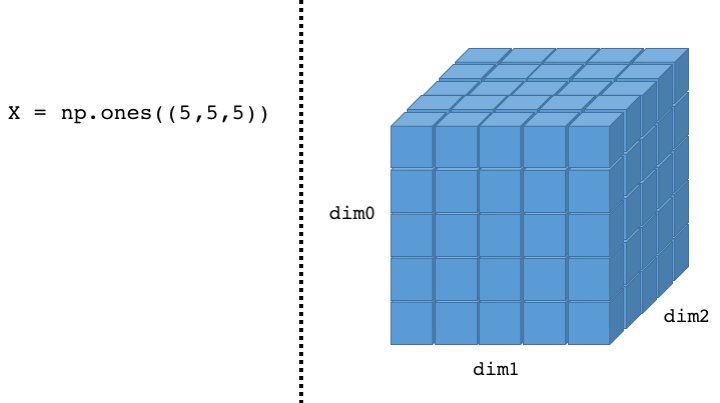
\includegraphics[width=4.5in]{{../Figures/array_slicing/Slide1}.png}
\end{frame}

\begin{frame}[t]{N-D Slicing}
	\centering
	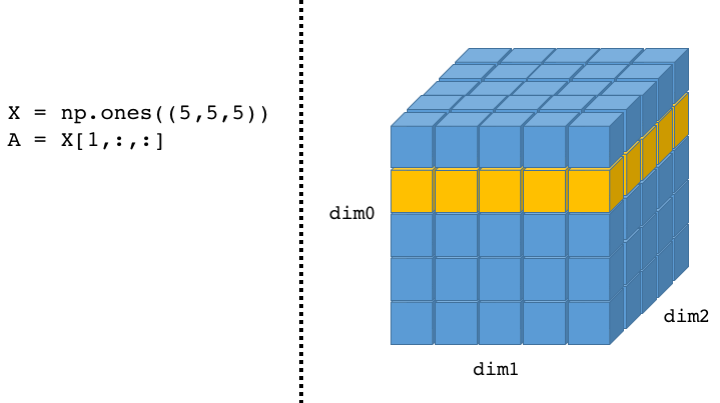
\includegraphics[width=4.5in]{{../Figures/array_slicing/Slide2}.png}
\end{frame}

\begin{frame}[t]{N-D Slicing}
	\centering
	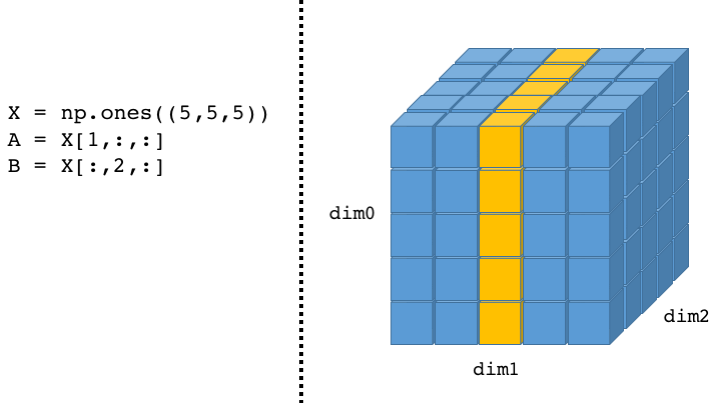
\includegraphics[width=4.5in]{{../Figures/array_slicing/Slide3}.png}
\end{frame}

\begin{frame}[t]{N-D Slicing}
	\centering
	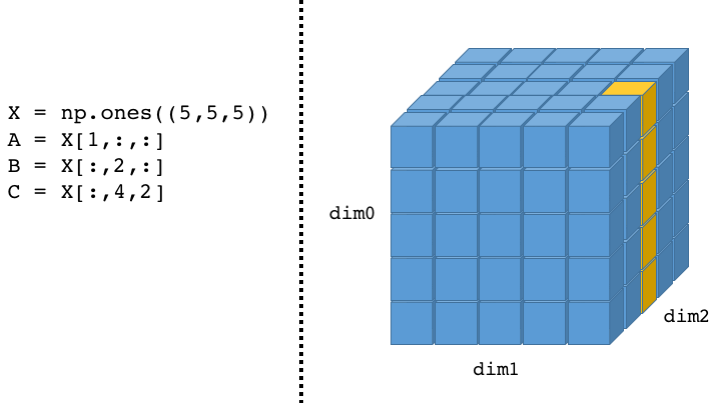
\includegraphics[width=4.5in]{{../Figures/array_slicing/Slide4}.png}
\end{frame}

\begin{frame}[t]{N-D Slicing}
	\centering
	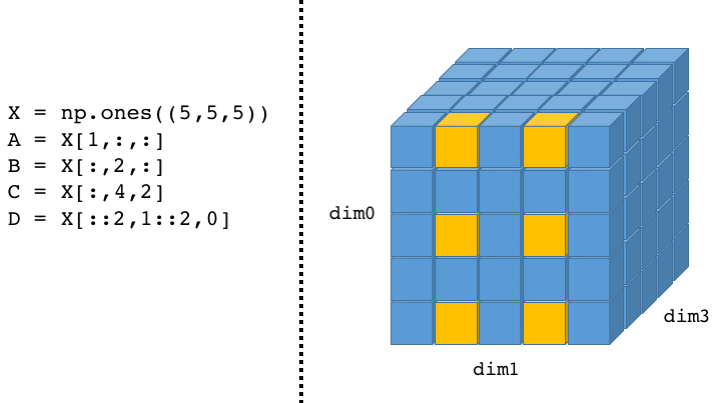
\includegraphics[width=4.5in]{{../Figures/array_slicing/Slide5}.png}
\end{frame}
	
\begin{frame}[t,fragile]{N-D Slicing}
	If a single index is passed for a dimension, the result will have one fewer dimensions than the original array.

	\begin{lstlisting}
		>>> a = np.ones((2,3,4))
		>>> a[:,1,:].shape
		(2,4)
	\end{lstlisting}
\end{frame}

\begin{frame}[t,fragile]{Entry/Slice Assignment}
	As with lists, we can assign to individual array entries or slices.

	\begin{lstlisting}
		>>> a = np.ones((3,3))
		>>> a[2,1] = 9
		>>> a
		array([[ 1.,  1.,  1.],
		       [ 1.,  1.,  1.],
		       [ 1.,  9.,  1.]]) 
		>>> a[:,0] = 5
		>>> a
		array([[ 5.,  1.,  1.],
		       [ 5.,  1.,  1.],
		       [ 5.,  9.,  1.]])
		>>> a[0,:] = np.arange(3)
		>>> a
		array([[ 0.,  1.,  2.],
		       [ 5.,  1.,  1.],
		       [ 5.,  9.,  1.]])
	\end{lstlisting}
\end{frame}

\begin{frame}[t,fragile]{Interactive Demo}
	\centering
	\Huge{Interactive Demo}
	\normalsize
	\begin{enumerate}
		\item Create an the following array:
		\begin{itemize}
			\item $a_j = 2^{3j} - j,\,\,j = 1,...,10$
		\end{itemize}
		\item \verb|np.all| and \verb|np.any| are NumPy functions that operate on boolean arrays. What do these functions do?
		\item How do you extract matrix $B$ from matrix $A$ with only indexing?
	\end{enumerate}
	
	$$ A = 
		\begin{bmatrix}
			1 & 2 & 3 & 4 & 5\\
			6 & 7 & 8 & 9 & 10\\
			11 & 12 & 13 & 14 & 15\\
			16 & 17 & 18 & 19 & 20\\
			21 & 22 & 23 & 24 & 25\\
		\end{bmatrix}\,\,\,\, B = 
		\begin{bmatrix}
			25 & 23 & 21\\
			15 & 13 & 11\\
			5 & 3 & 1\\
		\end{bmatrix}$$
	% 
\end{frame}

\begin{frame}[t,fragile]{Interactive Demo}
	\centering
	\Huge{Interactive Demo}
	\normalsize
	\begin{enumerate}
		\item Create an the following array:
		\begin{itemize}
			\item $a_j = 2^{3j} - j,\,\,j = 1,...,10$
			\item \verb|a = 2**(3*np.arange(1,11))-np.arange(1,11)|
		\end{itemize}
		\item \verb|np.all| and \verb|np.any| are NumPy functions that operate on boolean arrays. What do these functions do?
		\begin{itemize}
			\item \verb|np.all| returns \verb|True| if all elements of the array are true.
			\item \verb|np.any| returns \verb|True| if any elements of the array are true.
		\end{itemize}
		\item How do you extract matrix $B$ from matrix $A$ with only indexing?
		\begin{itemize}
			\item \verb|B = A[::-2,::-2]|
		\end{itemize}
	\end{enumerate}
	
	% $$ A =
	% 	\begin{bmatrix}
	% 		1 & 2 & 3 & 4 & 5\\
	% 		6 & 7 & 8 & 9 & 10\\
	% 		11 & 12 & 13 & 14 & 15\\
	% 		16 & 17 & 18 & 19 & 20\\
	% 		21 & 22 & 23 & 24 & 25\\
	% 	\end{bmatrix}\,\,\,\, B =
	% 	\begin{bmatrix}
	% 		25 & 23 & 21\\
	% 		15 & 13 & 11\\
	% 		5 & 3 & 1\\
	% 	\end{bmatrix}$$
	% 
\end{frame}

\end{document}
